% chapter: t3c files

\section{t3c files}

\subsection{file.t3c}
The file 'file.t3c' contains only one number, which gives the number of the NEXT file to write.
The number given here is the actual number of the file, if all files would be numbered from the beginning (including the initial file), starting with 0.
The file name though can be different (and is given in the 'mode.t3c'-file) and can contain any different number.

\subsection{init.t3c}
Null-point is in the frontal upper left corner of the grid.

\subsubsection{Grid parameter description}

The first part of 'init.t3c' describes some basic grid parameters:

\begin{table}[H]
\small
\centering
\begin{tabular}{p{3cm} p{6cm} p{3cm} l}
\toprule
Parameter & Description & Initial value & Unit\\
\midrule
xnumx & Number of nodes in x & $16N+5$ (4 multigrid levels) & - \\
ynumy & Number of nodes in y & $16N+5$ (4 multigrid levels) & - \\
znumz & Number of nodes in z & $16N+5$ (4 multigrid levels) & - \\
mnumx & Number markers per cell in x & - & - \\
mnumy & Number markers per cell in y & - & - \\
mnumz & Number markers per cell in z & - & - \\
xsize & Dimension of model in x & - & $[m]$ \\
ysize & Dimension of model in y & - & $[m]$ \\
zsize & Dimension of model in z & - & $[m]$ \\
pxinit & x-coordinate of initial pressure cell & $(xnumx-1)/2$ & - \\
pyinit & y-coordinate of initial pressure cell & $(ynumy-1)/2$ & - \\
pzinit & z-coordinate of initial pressure cell & - & - \\
pinit & Initial pressure in initial pressure cell & - & $[Pa]$ \\
GXKOEFF & Gravitational acceleration in x & - & $[m/s^2]$ \\
GYKOEFF & Gravitational acceleration in y & - & $[m/s^2]$ \\
GZKOEFF & Gravitational acceleration in z & - & $[m/s^2]$ \\
timesum & Starting time & - & $[years]$ \\
nonstab & number of random number generated & - &  \\
xnonstab & maximum random displacement of markers in x direction & - &  \\
ynonstab & maximum random displacement of markers in y direction & - &  \\
znonstab & maximum random displacement of markers in z direction & - &  \\
\footnotesize{markers types file name Y(Name) N(0)} & Number of initial output file & - & - \\
\footnotesize{data output file name} & Name of initial output file & name\_0.prn & - \\
TYPE	& type of data output & b (= binary), no other supported & - \\

\bottomrule
\end{tabular}
\caption{Grid parameter description}
\label{tbl:grid_parameter_description}
\end{table}

\subsubsection{Rock type description}

In the next part a table lists all possible types of material compositions together with their rheological properties.

\begin{table}[H]
\small
\centering
\begin{tabular}{l p{8cm} l}
\toprule
Parameter & Description & Unit\\
\midrule
rocknum & Rock number & - \\ 
markn0 & Individual lower viscosity limit & - \\ 
markn1 & Individual upper viscosity limit & - \\ 
marks0 & Connate water content at surface and surface temperature & $[wt\%]$ \\ 
marks1 & Individual upper stress limit & - \\ 
Nu or marknu & Newtonian viscosity & $[Pa^{MM}*s]$ \\ 
DE or markdh & Activation energy $E_a$ & $[J]$\\ 
DV or markdv & Activation volume $V_a$ & $[J/bar]$ \\ 
SS or markss & dislocation-diffusion transition stress $\sigma_{crit}$ & $[Pa]$ \\ 
MM or markmm & Stress exponent for creep law & $(Power)$ \\ 
LL or markll & Pore fluid pressure factor $1-\lambda$ (see eq.~\ref{eqs:mohr_coulomb}) & $(koef)$ \\ 
a0 or marka0 & Cohesion before cohesion weakening (see eq.~\ref{eqs:mohr_coulomb}) & $[Pa]$ \\
a1 or marka1 & Cohesion after cohesion weakening & - \\
b0 or markb0 & Sinus of effective internal friction angle in dry rock (see eq.~\ref{eqs:mohr_coulomb}) & [deg°]/[rad] \\
b1 or markb1 & sin$(\phi)$ after strain weakening & - \\
e0 or marke0 & Amount of strain marking beginning of strain weakening  & - \\
e1 or marke1 & Amount of strain marking the end of strain weakening  & - \\ 
RO or markro & Density & $[kg/M^3]$ \\ 
bb or bRo or markbb & Thermal expansion $\alpha$ (see eq.\ref{eqs:EOS}) & $[1/K]$ \\ 
aa or aRo or markaa & Compressibility $\beta$ (see eq.\ref{eqs:EOS}) & $[1/kbar]$\\ 
CP or markcp & Heat capacity  & $[J/kg]$ \\ 
Kt or markkt & Thermal conductivity & $[Wt/(m*K)]$ \\ 
Kf or markkf & Temperature dependency coefficient of conductivity & $[Wt/m]$ \\ 
Kp or markkp & Pressure dependency coefficient of conductivity & $[1/bar]$ \\ 
Ht & heat generation & $[Wt/kg]$\\ 
\bottomrule
\end{tabular}
\caption{Rock type parameters}
\label{tbl:rock_type_parameters}
\end{table}


\begin{table}[H]
\small
\centering
\begin{tabular}{l p{6cm} p{8cm}}
\toprule
Nr. & Description & Rheology\\
\midrule
\rowcolor[rgb]{1.0000    1.0000    1.0000}
00 & Air & -\\
\rowcolor[rgb]{0.5059    0.9961    0.7882}
01 & Water & -\\
\rowcolor[rgb]{1.0000    1.0000    1.0000}
02 & - &  - \\
\rowcolor[rgb]{0.6824    0.3412         0}
03 & Sediments 2 & WET QUARTZITE RANALLI 1995 \\
\rowcolor[rgb]{1.0000    0.5020         0}
04 & Sediments 3 & WET QUARTZITE RANALLI 1995 \\
\rowcolor[rgb]{0.7529    0.7529    0.7529}
05 & Upper Continental Crust & dry,felsic - WET QUARTZITE RANALLI 1995 \\
\rowcolor[rgb]{0.5020    0.5020    0.5020}
06 & Lower Continental Crust & dry,felsic - WET QUARTZITE RANALLI 1995 \\
\rowcolor[rgb]{ 0    0.5020         0}
07 & Upper Oceanic Crust & Basalts - WET QUARTZITE RANALLI 1995 \\
\rowcolor[rgb]{0    0.8431         0}
08 & Lower Oceanic Crust & Gabbro - An75 Ranalli1995 \\
\rowcolor[rgb]{0         0    0.7177}
09 & Lithospheric Mantle & dry peridotite - DRY OL Ranalli1995 \\
\rowcolor[rgb]{ 0.3216    0.2000    0.6745}
10 & Asthenospheric Mantle & dry peridotite - DRY OL Ranalli1995 \\
\rowcolor[rgb]{0.5412    0.7216    0.9922}
11 & Hydrated Mantle & wet peridotite - WET OL Ranalli1995 \\
\rowcolor[rgb]{0    0.5020    1.0000}
12 & Shear Zone & dry mantle peridotite - WET OL Ranalli1995 \\
\rowcolor[rgb]{0         0    0.4902}
13 & Serpentinized Mantle & wet peridotite \\
\rowcolor[rgb]{ 0.7000    0.1200    0.3000}
14 & Resolidified peridotite/ quenched mantle & dry peridotite \\
\rowcolor[rgb]{1.0000    1.0000    1.0000}
15 & - & - \\
\rowcolor[rgb]{0.3137    0.8941    0.2470}
16 & Newly formed crust & Basalt \\
\rowcolor[rgb]{0.5412    0.7216    0.9922}
17 & Hydrated Upper Crust & felsic - Hydrated WET QUARTZITE RANALLI 1995 \\
\rowcolor[rgb]{0.5412    0.7216    0.9922}
18 & Hydrated Lower Crust & felsic - Hydrated WET QUARTZITE RANALLI 1995 \\
\rowcolor[rgb]{1.0000    1.0000    1.0000}
19 & - & \\
\midrule
\rowcolor[rgb]{1.0000    1.0000    1.0000}
20 & - & \\
\rowcolor[rgb]{1.0000    1.0000    1.0000}
21 & - & \\
\rowcolor[rgb]{1.0000    1.0000    1.0000}
22 & - & - \\
\rowcolor[rgb]{1.0000    1.0000    0.3176}
23 & Partially molten Sediments 2 & \\
\rowcolor[rgb]{1.0000    0.9020    0.1882}
24 & Partially molten Sediments 3 & \\
\rowcolor[rgb]{0.4667    0.4667    0.2353}
25 & Partially molten Upper Continental Crust & felsic \\
\rowcolor[rgb]{0.5020    0.5020         0}
26 & Partially molten Lower Continental Crust & molten gabbro \\
\rowcolor[rgb]{0.7255    0.0157    0.7843}
27 & Partially molten Upper Oceanic Crust & molten basalt \\
\rowcolor[rgb]{0.9255    0.4392    0.9961}
28 & Partially molten Lower Oceanic Crust & molten gabbro \\
\rowcolor[rgb]{1.0000         0         0}
29 & Partially molten Lithospheric Mantle & dry peridotite \\
\rowcolor[rgb]{1.0000         0         0}
30 & Partially molten Asthenospheric Mantle & dry peridotite \\
\rowcolor[rgb]{1.0000    1.0000    1.0000}
31 & - & -\\
\rowcolor[rgb]{0.8471    0.0784    0.1529}
32 & Partially molten Shear Zone & dry peridotite \\
\rowcolor[rgb]{1.0000    1.0000    1.0000}
33 & - & -\\
\rowcolor[rgb]{1.0000         0         0}
34 & Partially molten Peridotite & \todo{dry or wet?} \\
\rowcolor[rgb]{1.0000    1.0000    1.0000}
35 & - & -\\
\rowcolor[rgb]{1.0000         0         0}
36 & Partially molten Newly Formed Crust & molten basalt \\
\rowcolor[rgb]{0.9922    0.3882    0.3020}
37 & Partially molten Hydrated Upper Crust & molten gabbro \\
\rowcolor[rgb]{0.9922    0.3882    0.3020}
38 & Partially molten Hydrated Lower Crust & molten gabbro \\
\midrule
+50	 & Water markers & \\
\midrule
+100 & External Composition & \\
\midrule
NAN & Undefined composition & black \\
\bottomrule
\end{tabular}
\caption{Rock types}
\label{tbl:rock_types}
\end{table}

Compositions 0-19 are all solids (except air and water). 20-39 are the equivalent melts. 50-89 are fluid markers. 100-139 are external compositions of the equivalent type, waiting outside the boundary to come into the model. They have the same properties as their internal equivalents.

\subsubsection{Boundary conditions}
Boundary conditions are prescribed separately for each of the six faces of the cube. Boundary conditions on each face don't have to be homogeneous.
Special 'open boundary conditions' can be prescribed, where e.g. the last marker gets 99\% of the velocity of the second to last and so on.

\begin{table}[H]
\small
\centering
\begin{tabular}{l l l}
\toprule
Parameter & Description & Range of values \\
\midrule
Val & BC type & P, Vx, Vy, Vz, T, X, Y, Z, M \\
m10 & starting node position in x &  \\ 
m11 & ending node position in x &  \\ 
m20 & starting node position in y &  \\ 
m21 & ending node position in y &  \\ 
m30 & starting node position in z. &  \\ 
m31 & ending node position in z &  \\ 
Const & boundary value &  \\ 
Koef &  multiplier for boundary velocity & [0,1] \\ 
nshiftx & determines which x-node is used to calculate value at next node & -1, +0 or +1 \\ 
nshifty & determines which y-node is used to calculate value at next node & -1, +0 or +1 \\ 
nshiftz & determines which z-node is used to calculate value at next node & -1, +0 or +1 \\ 
Koef1 &  &  \\ 
nshiftx1 & Ignored if Koef1 is 0 &  \\ 
nshifty1 & Ignored if Koef1 is 0 &  \\ 
nshiftz1 & Ignored if Koef1 is 0 &  \\ 
Koef2 &  &  \\ 
nshiftx2 & Ignored if Koef2 is 0 &  \\ 
nshifty2 & Ignored if Koef2 is 0 &  \\ 
nshiftz2 & Ignored if Koef2 is 0 &  \\ 
\bottomrule
\end{tabular}
\caption{Boundary condition parameters}
\label{tbl:BC_parameters}
\end{table}

\paragraph{P, Vx, Vy, Vz, T boundary conditions}
For all nodes in the given range $[m10,m11]\times[m20,m21]\times[m30,m31]$ the following boundary condition is applied:
\begin{equation}\label{eqs:PVT_BC_general}
A(x,y,z) = Const + Koef \cdot A(x+nshiftx,y+nshifty,z+nshiftz)
\end{equation}

E.g. the following part in the \textit{init.t3c} file:
\begin{lstlisting}
/Left_Bondary
/Val___m10_m11___m20_m21___m30_m31___Const___Koef_dm1_dm2_dm3
 Vx____0___0_____0___y-1___0___z-1___3e-10___0____0___0___0
\end{lstlisting}
translates into the following boundary condition:
\begin{equation}
V_x(x,y,z) = 3\times10^{-10} \quad \mid x=0, y\in[0,y-1], z\in[0,z-1]
\end{equation}

\paragraph{X, Y, Z coordinates definition}
For all nodes in the given range $[m10,m11]\times[m20,m21]\times[m30,m31]$ the following equation is applied, shown at the example of the x-grid:

\begin{subequations}
\begin{equation}\label{eqs:XYZ_BC_general}
X(x,y,z) = X(x-1,y,z) + Const + (Koef-Const) \cdot \dfrac{(x-m10)}{(m11-m10)} \quad \mid Koef1=0
\end{equation}
\begin{equation}
X(x,y,z) = X(x-1,y,z) + exp{\left(log{\left(Const\right)}+log{\left(\dfrac{Koef1}{Const}\right)}\right)} \cdot \dfrac{(x-m10)}{(m11-m10)}
\end{equation}
\end{subequations}

\paragraph{M marker grid set to cell}
For all nodes in the given range $[m10,m11]\times[m20,m21]\times[m30,m31]$ additional markers are added. All parameters ($Koef$, $Koef1$, $Koef2$, $nshiftx$, $nshiftx1$,..,$nshiftz1$,$nshiftz2$) need to be set. $nshiftx$ gives the shift in $x$, $nshifty1$ gives the shift in $y$, $nshiftz2$ gives the shift in $z$ and all other shift parameters are ignored. If $Koef$ is set, random nonstability is set on the new marker field in $X$ in the following way:
\begin{equation}\label{eqs:M_BC_general}
markx= x + \dfrac{rand() \% \left(\lfloor Const \rfloor *2+1\right)-\lfloor Const \rfloor}{Const} \cdot \dfrac{X(x+1,y,z)-X(x,y,z)}{nshiftx}\cdot Koef
\end{equation}
Random nonstability is set in $Y$ for $Koef1>0$ and in $Z$ for $Koef2>0$ in the same way.

\subsubsection{Box description}
Arbitrary shapes of cubes are prescribed by setting the (x,y,z) coordinate of each of the 8 corners (Figure \ref{fig:cube}).

\begin{figure}
    \centering
    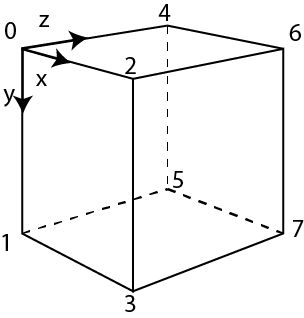
\includegraphics{Illustrations/i3elviscube.png}
    \caption{Illustration of the faces of the cube referred to in Tables \ref{tbl:box_parameters} and \ref{tbl:t_box_parameters}.}
    \label{fig:cube}
\end{figure}

\begin{table}[H]
\centering
\begin{tabular}{l l l}
\toprule
Parameter		& Description			& Range of value \\
\midrule
Type			& Rock type				& $0-140$\\
$[x_0,y_0,z_0]$ & front upper left\\ 
$[x_1,y_1,z_1]$ & front lower left \\  
$[x_2,y_2,z_2]$ & front upper right \\ 
$[x_3,y_3,z_3]$ & front lower right \\ 
$[x_4,y_4,z_4]$ & back upper left \\  
$[x_5,y_5,z_5]$ & back lower left \\ 
$[x_6,y_6,z_6]$ & back upper right \\  
$[x_7,y_7,z_7]$ & back lower right \\ 
\bottomrule
\end{tabular}
\caption{Box parameters}
\label{tbl:box_parameters}
\end{table}

Coordinates can be given either relative [0,1], or absolute [m0, mMAXSIZE], where MAXSIZE cannot be larger than the maximum domain size in this direction. With the leading 'm', the value is interpreted as an absolute value in meters.

e.g.
\begin{lstlisting}
/Type=RockType
/Type__x0__y0__z0___x1__y1__z1_____x2__y2__z2_____x3__y3__z3
/_____x4__y4__z4___x5__y5__z5_____x6__y6__z6______x7__y7__z7
/Asthenosphere
10____0_m15000_0___0__1.1__0_____1.1_m15000_0_____1.1_1.1__0
______0_m15000_1___0__1.1__1_____1.1_m15000_1_____1.1_1.1__1
\end{lstlisting}

\subsubsection{Temperature box description}
Arbitrary shapes of cubes are prescribed by setting the (x,y,z) coordinate of each of the 8 corners (Figure \ref{fig:cube}).

\begin{table}[H]
\centering
\begin{tabular}{l l}
\toprule
Parameter		& Description\\
\midrule
Type			& Box type: $0$ - simple box; $1\&4$ - age box; $5\&6$ - transitional\\
$[x_0,y_0,z_0]$ & front upper left\\
$[x_1,y_1,z_1]$ & front lower left with $x_1=x_0$, $z_1=z_0$\\
$[x_2,y_2,z_2]$ & front upper right with $z_2=z_0$\\ 
$[x_3,y_3,z_3]$ & front lower right with $x_3=x_2$, $z_3=z_0$\\ 
$[x_4,y_4,z_4]$ & back upper left with $x_4=x_5$, $z_4=z_7$\\  
$[x_5,y_5,z_5]$ & back lower left with $z_4=z_7$\\ 
$[x_6,y_6,z_6]$ & back upper right with $x_6=x_7$, $z_6=z_7$\\
$[x_7,y_7,z_7]$ & back lower right\\
$t_0$ & simple box: temperature $P_0$; age box: surface temperature\\
$t_1$ & simple box: temperature $P_1$; age box: initial temperature\\
$t_2$ & simple box: temperature $P_2$; age box: thermal diffusivity $\kappa$ in $P_0$\\
$t_3$ & simple box: temperature $P_3$; age box: thermal diffusivity $\kappa$ in $P_2$\\
$t_4$ & simple box: temperature $P_4$; age box: thermal diffusivity $\kappa$ in $P_4$\\
$t_5$ & simple box: temperature $P_5$; age box: thermal diffusivity $\kappa$ in $P_6$\\
$t_6$ & simple box: temperature $P_6$; age box: characteristic diffusion time\\
$t_7$ & simple box: temperature $P_7$; age box: overprinted linear geotherm $[\degree/m]$\\
\bottomrule
\end{tabular}
\caption{Temperature box parameters}
\label{tbl:t_box_parameters}
\end{table}

Coordinates can be given either relative [0,1], or absolute [m0, mMAXSIZE], where MAXSIZE cannot be larger than the maximum domain size in this direction. With the leading 'm', the value is interpreted as an absolute value in meters.

\paragraph{Box type 0: simple box}
The given temperatures are set to the given coordinates and temperature is interpolated linearly within the box.

\paragraph{Box type 1\&4: age box}
Within the given coordinates the temperature is given by conductive cooling in the following way:
\begin{equation}\label{eqs:cond_cooling}
T(y,t)=T_1-(1-erf(\dfrac{y}{2\sqrt{\kappa\tau}}))(T_1-T_0),
\end{equation}
where $\kappa=\dfrac{k}{\rho c_p}$ is the thermal diffusivity interpolated over the corner of the box and $\tau=\dfrac{l^2}{\kappa}$ is the characteristic diffusion time.

\paragraph{Box type 5\&6: transitional box}
No new temperatures are set but existing temperatures at the coordinates of the box corners are read. Those are then interpolated linearly through out the box.

E.g. the continental crust and lithosphere is modelled in a simple box by a geothermal gradient of $\sim17\,K/km$ spanning the whole width of the model and starting at $12\,km$ depth with a surface temperature of $273\,K$, going down to a depth of $90\,km$:
\lstset{basicstyle=\small}
\begin{lstlisting}
/T_BOXES_DESCRIPTION
/Typ__x0________x2_______y0________y1_______y2_______y3_______z0_______
	_x5_______x7_______y4_______y5_______y6_______y7_______z7_______
	t0___t1___t2___t3___t4___t5___t6___t7
/Oceanic_and_continental_geotherms
0    -0.000001 m350001  m12000    m90000   m12000    m90000 -0.000001
	-0.000001 m350001  m12000    m90000  m12000    m90000  1.000001
	273  1595 273  1595 273  1595 273  1595
\end{lstlisting}

\subsection{mode.t3c}

\subsubsection{Timestepping description}

The first/second line gives the filename and type of the initial file.

In the next very large block one timestep corresponds with one line and the data is only valid for one timestep. Seperate timestep parameters are given in table~\ref{tbl:timestep_parameters}.

\begin{table}[H]
\small
\centering
\begin{tabular}{l p{13cm}}
\toprule
Parameter & Description \\
\midrule
SAVEFILE & name of the file (if this name is non-unique, the file will be overwritten without warning) \\
TYPE & file type: b = binary (no other supported) \\
cyc0max & number of iterations \\
maxxystep & maximum change in x,y,z in one timestep  \\
maxtkstep & maximum step size in temperature \ \\
maxtmstep & maximum step size in time \\
nubeg & global lower viscosity cut-off \\
nuend & global upper viscosity cut-off \\
p0koef & Pressure penalty factor 1, Relaxation parameter in Continuity equation \\
p1koef & Pressure update interpolation from coarser multigrid levels \\
p2koef & Pressure penalty factor 2 \todo{???} \\
unused & - \\
multinum &  number of multigrid levels \\
stp1 & number of iterations/ repeats for whole timestep \\
multinum2 & number of multigrid levels 2 \todo{???} \\
\bottomrule
\end{tabular}
\caption{Timestep parameters}
\label{tbl:timestep_parameters}
\end{table}

\subsubsection{General parameters}
The following parameters are mainly used to control the general behaviour of the program.

\begin{table}[H]
\small
\centering
\begin{tabular}{l p{11cm} l}
\toprule
Parameter & Description & Default \\
\midrule
\pcode{loadmod		}&\pcode{ load from data file (1) or set initial conditions (0) }&\pcode{ 1}\\
printmod 	& print information on the monitor, Yes (1)/ No (2) & 1\\
\pcode{crustmod	}&\pcode{ print information on crustthickness in files for each nth timestep; 0 = disable }&\pcode{ - }\\
\pcode{dynamod		}&\pcode{ do dynamo calculations for each nth timestep; 0 = disabled }&\pcode{ - }\\
\pcode{fl0num 		}&\pcode{ number of otput file Names }&\pcode{ - }\\
movemod 	& do velocity-pressure iterations, solve continuity and Stokes equation & 1\\
tempmod 	& do temperature iterations, solve heat transfer equation & 1\\
markmod 	& move markers Y(1-simple,2-Runge-Kutta4)/N(0) & 2\\
gridmod 	& recalculate density and viscosity & 1\\
outgrid 	& marker move out of grid Y(0)/N(1) Orthogonal Only (2) & 2\\
densimod	& mode of  density calculation: 0-constant, 1-PT-dependent, 2-TDbase 3-PT-dependent+WaterTDbase & 3 \\
stp100 		& \todo{???} & 9000 \\
\pcode{CTreset 	}&\pcode{ composition/temperature reset for water/air at $100\,km$ above surface Y(1)/N(0) }&\pcode{ 1 }\\
\pcode{smeltextract}&\pcode{ extract melt when moving markers Y(1)/N(0) } & \pcode{1}\\
\pcode{sthdatabase }&\pcode{ Use of Mars thermodynamic database Y(1) or standard database N(0) } & \pcode{1}\\
p2vmod		& convert each nth prn to vtr /N(0) & 10 \\
filestop 	& number of timesteps to execute before exiting & 50\\
\bottomrule
\end{tabular}
\caption{General parameters}
\label{tbl:mode_general_parameters}
\end{table}

\subsubsection{Erosion and Sedimentation parameters}

\begin{table}[H]
\small
\centering
\begin{tabular}{l p{10cm} l}
\toprule
Parameter & Description & Initial value \\
\midrule
eroslev 	& Erosion level: markers above this depth which are neither sticky air nor water get converted to sticky air & 8000\\
sedilev 	& Sedimentation level: sticky air or water below this depth gets converted to sediments & 20000\\
waterlev 	& Water level: sticky air markers below water level are converted to water and water markers above water level are converted to sticky air & 12000\\
\bottomrule
\end{tabular}
\caption{Erosion and Sedimentation parameters}
\label{tbl:mode_sed_parameters}
\end{table}

\subsubsection{Velocity- and Pressure-iterations parameters}
The following parameters are mainly needed to solve the Continuity and Stokes equation with multigrid. Some these parameters already appeared in table~\ref{tbl:timestep_parameters} and their global value given here will be overwritten with the new value for each timestep. 

\begin{table}[H]
\small
\centering
\begin{tabular}{l p{9cm} p{3cm}}
\toprule
Parameter & Description & Initial value \\
\midrule
cyc1max 	& unused & $3000$\\
DIVVMIN 	& Continuity equation lower error bound & $3e{-03}$\\
STOKSMIN 	& Stokes equation lower error bound & $5e{+01}$\\
DIVVMAX 	& Continuity equation upper error bound & $0e{-03}$\\
STOKSMAX 	& Stokes equation upper error bound & $3e{-03}$\\
multinum 	& number of multigrid levels; overwritten by separate timestep value & $4$\\
multicyc	& Number of whole multigrid V-cycle iterations & $1$ \\
multinnn 	& V-cycle structure: number of GS-iterations for each multigrid level in upcycle and downcycle. & $4\,16\,16\,32\,0$; $4\,16\,16\,32\,64$\\
p0koef 		& Global pressure penalty factor 1, Relaxation parameter in Continuity equation; overwritten by separate timestep value & $3.0e{-01}$\\
p1koef 		& Global pressure update interpolation from coarser multigrid level; overwritten by separate timestep value & $1.0e{-00}$\\
p2koef 		& Global pressure penalty factor 2 \todo{???}; overwritten by separate timestep value & $0.0e{-00}$\\
v0koef 		& Velocity penalty facto. Relaxation parameter in vx-,vy-,vz-Stokes equation & $1.0e{-00}$\\
v1koef 		& \todo{???} & $1.0e{-00}$\\
nubeg 		& global lower viscosity cut-off; overwritten by separate timestep value & $1e{+18}$\\
nuend 		& global upper viscosity cut-off; overwritten by separate timestep value & $1e{+25}$\\
nukoef 		& Average $\nu$ for pressure optimisation & $0.0$\\
viscmod 	& Effective viscosity mode. 0 = lin. interp; 1 = exp. interp; 2 = inverse interp; & $0$\\
\pcode{viscoutermod}&\pcode{viscosity in space/air/water; 1-gradual increase in space, 2-gradual increase in water/air}&\pcode{ $2$}\\
\pcode{spheryn 	}&\pcode{ Spherical gravity. 0 = off; 1 = on; }&\pcode{ $0$}\\
\bottomrule
\end{tabular}
\caption{V and P iterations parameters}
\label{tbl:mode_v_p_parameters}
\end{table}

\paragraph{viscmod: Effective viscosity interpolation}
Type of interpolation done to obtain effective viscosity. viscmod = 0 uses linear interpolation (eq.~\ref{eqs:viscmod0}), viscmod = 1 uses exponential interpolation (eq.~\ref{eqs:viscmod1}) and viscmod = 2 uses inverse interpolation (eq.~\ref{eqs:viscmod2}).
\begin{subequations}
\begin{equation}\label{eqs:viscmod0}
\eta_{eff}=\dfrac{1}{8}\sum_{i}\eta_i
\end{equation}
\begin{equation}\label{eqs:viscmod1}
\eta_{eff}=exp{\left(\dfrac{1}{8}\sum_{i}\left(log\left(\eta_i\right)\right)\right)}
\end{equation}
\begin{equation}\label{eqs:viscmod2}
\eta_{eff}=\dfrac{1}{\frac{1}{8}\sum\limits_{i}{\frac{1}{\eta_i}}}
\end{equation}
\end{subequations}

\subsubsection{Temperature-iterations parameters}
The following parameters are mainly needed to solve the temperature equation with multigrid.

\begin{table}[H]
\small
\centering
\begin{tabular}{l p{9cm} l}
\toprule
Parameter & Description & Initial value \\
\midrule
cyc2max 	& unused & $2500$\\
HEATMIN 	& Temperature equation lower error bound & $1e{-4}$\\
multinumt 	& Number of multigrid levels & $0$\\
multicyct 	& Number of whole multigrid V-cycle iterations & $1$ \\
multittt	& V-cycle structure: number of GS-iterations for each multigrid level in upcycle and downcycle & $1$; $0$ \\
t0koef 		& \todo{???} & $1.0e{-00}$\\
t1koef 		& \todo{???} & $1.0e{-00}$\\
heatdif 	& \todo{???} & $1.0$\\
frictyn 	& \todo{???} & $1$\\
adiabyn 	& \todo{???} & $1$\\
\bottomrule
\end{tabular}
\caption{T iterations parameters}
\label{tbl:mode_t_parameters}
\end{table}

\subsubsection{Hydration and melting parameters}

\begin{table}[H]
\small
\centering
\begin{tabular}{l p{7cm} l}
\toprule
Parameter & Description & Initial value \\
\midrule
tkpor 		& Maximum temperature for porosity & $97300000.0$\\
zmpor 		& Maximum depth for porosity & $75000$\\
vyfluid 	& Initial fluid velocity & $-3e{-09}$\\
vymelt 		& Initial melt velocity & $-3e{-09}$\\
dmwamin 	& Minimum water release difference & $1e{-1}$\\
tdeep 		& \todo{???} & $1880.0$\\
dtdeep 		& \todo{???} & $100.0$\\
drdeep 		& \todo{???} & $000.0$\\
zdeep 		& \todo{???} & $660000.0$\\
vdeep		& \todo{???} & $670000.0$\\
nudeep		& \todo{???} & $1e{+21}$\\
dxwater		& Fluid extension in x & $2e{+3}$\\
dywater		& Fluid extension in y & $2e{+3}$\\
dzwater		& Fluid extension in z & $2e{+3}$\\
maxwater	& Maximum water content in peridotite melt & $5e{-1}$\\
minmelt		& \todo{???} & $1e{-2}$\\
maxmelt		& \todo{???} & $1e{-2}$\\
maxpmelt	& Maximum pressure for dry mantle melting & \\
\bottomrule
\end{tabular}
\caption{Hydration and melting parameters}
\label{tbl:mode_melting_parameters}
\end{table}

\subsubsection{Collision velocity parameters}

Linearly change collision velocity. Use initial constant velocity set from boundary conditions. Between \emph{timebeg} and \emph{timeend} linearly change the collision velocity to the final velocity \emph{velocitykf}.

\begin{table}[H]
\small
\centering
\begin{tabular}{l l l}
\toprule
Parameter & Description & Initial value \\
\midrule
timebeg 	& Begin velocity change & $20e{+6}$\\
timeend 	& End velocity change & $25e{+6}$\\
velocitykf 	& Final collision velocity & $0$\\
\bottomrule
\end{tabular}
\caption{Collision velocity parameters}
\label{tbl:mode_collision_parameters}
=======
% chapter: t3c files

\section{t3c files}

\subsection{file.t3c}
The file 'file.t3c' contains only one number, which gives the number of the NEXT file to write.
The number given here is the actual number of the file, if all files would be numbered from the beginning (including the initial file), starting with 0.
The file name though can be different (and is given in the 'mode.t3c'-file) and can contain any different number.

\subsection{init.t3c}
Null-point is in the frontal upper left corner of the grid.

\subsubsection{Grid parameter description}

The first part of 'init.t3c' describes some basic grid parameters:

\begin{table}[H]
\small
\centering
\begin{tabular}{p{3cm} p{6cm} p{3cm} l}
\toprule
Parameter & Description & Initial value & Unit\\
\midrule
xnumx & Number of nodes in x & $16N+5$ (4 multigrid levels) & - \\
ynumy & Number of nodes in y & $16N+5$ (4 multigrid levels) & - \\
znumz & Number of nodes in z & $16N+5$ (4 multigrid levels) & - \\
mnumx & Number markers per cell in x & - & - \\
mnumy & Number markers per cell in y & - & - \\
mnumz & Number markers per cell in z & - & - \\
xsize & Dimension of model in x & - & $[m]$ \\
ysize & Dimension of model in y & - & $[m]$ \\
zsize & Dimension of model in z & - & $[m]$ \\
pxinit & x-coordinate of initial pressure cell & $(xnumx-1)/2$ & - \\
pyinit & y-coordinate of initial pressure cell & $(ynumy-1)/2$ & - \\
pzinit & z-coordinate of initial pressure cell & - & - \\
pinit & Initial pressure in initial pressure cell & - & $[Pa]$ \\
GXKOEFF & Gravitational acceleration in x & - & $[m/s^2]$ \\
GYKOEFF & Gravitational acceleration in y & - & $[m/s^2]$ \\
GZKOEFF & Gravitational acceleration in z & - & $[m/s^2]$ \\
timesum & Starting time & - & $[years]$ \\
nonstab & number of random number generated & - &  \\
xnonstab & maximum random displacement of markers in x direction & - &  \\
ynonstab & maximum random displacement of markers in y direction & - &  \\
znonstab & maximum random displacement of markers in z direction & - &  \\
\footnotesize{markers types file name Y(Name) N(0)} & Number of initial output file & - & - \\
\footnotesize{data output file name} & Name of initial output file & name\_0.prn & - \\
TYPE	& type of data output & b (= binary), no other supported & - \\

\bottomrule
\end{tabular}
\caption{Grid parameter description}
\label{tbl:grid_parameter_description}
\end{table}

\subsubsection{Rock type description}

In the next part a table lists all possible types of material compositions together with there rheological properties.

\begin{table}[H]
\small
\centering
\begin{tabular}{l p{8cm} l}
\toprule
Parameter & Description & Unit\\
\midrule
rocknum & Rock number & - \\ 
markn0 & Individual lower viscosity limit & - \\ 
markn1 & Individual upper viscosity limit & - \\ 
marks0 & Connate water content at surface and surface temperature & $[wt\%]$ \\ 
marks1 & Individual upper stress limit & - \\ 
Nu or marknu & Newtonian viscosity & $[Pa^{MM}*s]$ \\ 
DE or markdh & Activation energy $E_a$ & $[J]$\\ 
DV or markdv & Activation volume $V_a$ & $[J/bar]$ \\ 
SS or markss & dislocation-diffusion transition stress $\sigma_{crit}$ & $[Pa]$ \\ 
MM or markmm & Stress exponent for creep law & $(Power)$ \\ 
LL or markll & Pore fluid pressure factor $1-\lambda$ (see eq.~\ref{eqs:mohr_coulomb}) & $(koef)$ \\ 
a0 or marka0 & Cohesion (see eq.~\ref{eqs:mohr_coulomb}) & $[Pa]$ \\
a1 or marka1 & unused & - \\
b0 or markb0 & Sinus of effective internal friction angle in dry rock (see eq.~\ref{eqs:mohr_coulomb}) & [deg°]/[rad] \\
b1 or markb1 & unused & - \\
e0 or marke0 & Koef in ductile rheology weakening \todo{???} & \todo{???} \\
e1 or marke1 & Koef in ductile rheology weakening \todo{???} & \todo{???} \\ 
RO or markro & Density & $[kg/M^3]$ \\ 
bb or bRo or markbb & Thermal expansion $\alpha$ (see eq.\ref{eqs:EOS}) & $[1/K]$ \\ 
aa or aRo or markaa & Compressibility $\beta$ (see eq.\ref{eqs:EOS}) & $[1/kbar]$\\ 
CP or markcp & Heat capacity  & $[J/kg]$ \\ 
Kt or markkt & Thermal conductivity & $[Wt/(m*K)]$ \\ 
Kf or markkf & Temperature dependency coefficient of conductivity & $[Wt/m]$ \\ 
Kp or markkp & Pressure dependency coefficient of conductivity & $[1/bar]$ \\ 
Ht & heat generation & $[Wt/kg]$\\ 
\bottomrule
\end{tabular}
\caption{Rock type parameters}
\label{tbl:rock_type_parameters}
\end{table}


\begin{table}[H]
\small
\centering
\begin{tabular}{l p{6cm} p{8cm}}
\toprule
Nr. & Description & Rheology\\
\midrule
\rowcolor[rgb]{1.0000    1.0000    1.0000}
00 & Air & -\\
\rowcolor[rgb]{0.5059    0.9961    0.7882}
01 & Water & -\\
\rowcolor[rgb]{1.0000    1.0000    1.0000}
02 & - &  - \\
\rowcolor[rgb]{0.6824    0.3412         0}
03 & Sediments 2 & WET QUARTZITE RANALLI 1995 \\
\rowcolor[rgb]{1.0000    0.5020         0}
04 & Sediments 3 & WET QUARTZITE RANALLI 1995 \\
\rowcolor[rgb]{0.7529    0.7529    0.7529}
05 & Upper Continental Crust & dry,felsic - WET QUARTZITE RANALLI 1995 \\
\rowcolor[rgb]{0.5020    0.5020    0.5020}
06 & Lower Continental Crust & dry,felsic - WET QUARTZITE RANALLI 1995 \\
\rowcolor[rgb]{ 0    0.5020         0}
07 & Upper Oceanic Crust & Basalts - WET QUARTZITE RANALLI 1995 \\
\rowcolor[rgb]{0    0.8431         0}
08 & Lower Oceanic Crust & Gabbro - An75 Ranalli1995 \\
\rowcolor[rgb]{0         0    0.7177}
09 & Lithospheric Mantle & dry peridotite - DRY OL Ranalli1995 \\
\rowcolor[rgb]{ 0.3216    0.2000    0.6745}
10 & Asthenospheric Mantle & dry peridotite - DRY OL Ranalli1995 \\
\rowcolor[rgb]{0.5412    0.7216    0.9922}
11 & Hydrated Mantle & wet peridotite - WET OL Ranalli1995 \\
\rowcolor[rgb]{0    0.5020    1.0000}
12 & Shear Zone & dry mantle peridotite - WET OL Ranalli1995 \\
\rowcolor[rgb]{0         0    0.4902}
13 & Serpentinized Mantle & wet peridotite \\
\rowcolor[rgb]{ 0.7000    0.1200    0.3000}
14 & Resolidified peridotite/ quenched mantle & dry peridotite \\
\rowcolor[rgb]{1.0000    1.0000    1.0000}
15 & - & - \\
\rowcolor[rgb]{0.3137    0.8941    0.2470}
16 & Newly formed crust & Basalt \\
\rowcolor[rgb]{0.5412    0.7216    0.9922}
17 & Hydrated Upper Crust & felsic - Hydrated WET QUARTZITE RANALLI 1995 \\
\rowcolor[rgb]{0.5412    0.7216    0.9922}
18 & Hydrated Lower Crust & felsic - Hydrated WET QUARTZITE RANALLI 1995 \\
\rowcolor[rgb]{1.0000    1.0000    1.0000}
19 & - & \\
\midrule
\rowcolor[rgb]{1.0000    1.0000    1.0000}
20 & - & \\
\rowcolor[rgb]{1.0000    1.0000    1.0000}
21 & - & \\
\rowcolor[rgb]{1.0000    1.0000    1.0000}
22 & - & - \\
\rowcolor[rgb]{1.0000    1.0000    0.3176}
23 & Partially molten Sediments 2 & \\
\rowcolor[rgb]{1.0000    0.9020    0.1882}
24 & Partially molten Sediments 3 & \\
\rowcolor[rgb]{0.4667    0.4667    0.2353}
25 & Partially molten Upper Continental Crust & felsic \\
\rowcolor[rgb]{0.5020    0.5020         0}
26 & Partially molten Lower Continental Crust & molten gabbro \\
\rowcolor[rgb]{0.7255    0.0157    0.7843}
27 & Partially molten Upper Oceanic Crust & molten basalt \\
\rowcolor[rgb]{0.9255    0.4392    0.9961}
28 & Partially molten Lower Oceanic Crust & molten gabbro \\
\rowcolor[rgb]{1.0000         0         0}
29 & Partially molten Lithospheric Mantle & dry peridotite \\
\rowcolor[rgb]{1.0000         0         0}
30 & Partially molten Asthenospheric Mantle & dry peridotite \\
\rowcolor[rgb]{1.0000    1.0000    1.0000}
31 & - & -\\
\rowcolor[rgb]{0.8471    0.0784    0.1529}
32 & Partially molten Shear Zone & dry peridotite \\
\rowcolor[rgb]{1.0000    1.0000    1.0000}
33 & - & -\\
\rowcolor[rgb]{1.0000         0         0}
34 & Partially molten Peridotite & \todo{dry or wet?} \\
\rowcolor[rgb]{1.0000    1.0000    1.0000}
35 & - & -\\
\rowcolor[rgb]{1.0000         0         0}
36 & Partially molten Newly Formed Crust & molten basalt \\
\rowcolor[rgb]{0.9922    0.3882    0.3020}
37 & Partially molten Hydrated Upper Crust & molten gabbro \\
\rowcolor[rgb]{0.9922    0.3882    0.3020}
38 & Partially molten Hydrated Lower Crust & molten gabbro \\
\midrule
+50	 & Water markers & \\
\midrule
+100 & External Composition & \\
\midrule
NAN & Undefined composition & black \\
\bottomrule
\end{tabular}
\caption{Rock types}
\label{tbl:rock_types}
\end{table}

Compositions 0-19 are all solids (except air and water). 20-39 are the equivalent melts. 50-89 are fluid markers. 100-139 are external compositions of the equivalent type, waiting outside the boundary to come into the model. They have the same properties as their internal equivalents.

\subsubsection{Boundary conditions}
Boundary conditions are prescribed separately for each of the six faces of the cube. Boundary conditions on each face don't have to be homogeneous.
Special 'open boundary conditions' can be prescribed, where e.g. the last marker gets 99\% of the velocity of the second to last and so on.

\begin{table}[H]
\small
\centering
\begin{tabular}{l l l}
\toprule
Parameter & Description & Range of values \\
\midrule
Val & BC type & P, Vx, Vy, Vz, T, X, Y, Z, M \\
m10 & starting node position in x &  \\ 
m11 & ending node position in x &  \\ 
m20 & starting node position in y &  \\ 
m21 & ending node position in y &  \\ 
m30 & starting node position in z. &  \\ 
m31 & ending node position in z &  \\ 
Const &  &  \\ 
Koef &  &  \\ 
nshiftx &  &  \\ 
nshifty &  &  \\ 
nshiftz &  &  \\ 
Koef1 &  &  \\ 
nshiftx1 & Ignored if Koef1 is 0 &  \\ 
nshifty1 & Ignored if Koef1 is 0 &  \\ 
nshiftz1 & Ignored if Koef1 is 0 &  \\ 
Koef2 &  &  \\ 
nshiftx2 & Ignored if Koef2 is 0 &  \\ 
nshifty2 & Ignored if Koef2 is 0 &  \\ 
nshiftz2 & Ignored if Koef2 is 0 &  \\ 
\bottomrule
\end{tabular}
\caption{Boundary condition parameters}
\label{tbl:BC_parameters}
\end{table}

\paragraph{P, Vx, Vy, Vz, T boundary conditions}
For all nodes in the given range $[m10,m11]\times[m20,m21]\times[m30,m31]$ the following boundary condition is applied:
\begin{equation}\label{eqs:PVT_BC_general}
A(x,y,z) = Const + Koef \cdot A(x+nshiftx,y+nshifty,z+nshiftz)
\end{equation}

E.g. the following part in the \textit{init.t3c} file:
\begin{lstlisting}
/Left_Bondary
/Val___m10_m11___m20_m21___m30_m31___Const___Koef_dm1_dm2_dm3
 Vx____0___0_____0___y-1___0___z-1___3e-10___0____0___0___0
\end{lstlisting}
translates into the following boundary condition:
\begin{equation}
V_x(x,y,z) = 3\times10^{-10} \quad \mid x=0, y\in[0,y-1], z\in[0,z-1]
\end{equation}

\paragraph{X, Y, Z coordinates definition}
For all nodes in the given range $[m10,m11]\times[m20,m21]\times[m30,m31]$ the following equation is applied, shown at the example of the x-grid:

\begin{subequations}
\begin{equation}\label{eqs:XYZ_BC_general}
X(x,y,z) = X(x-1,y,z) + Const + (Koef-Const) \cdot \dfrac{(x-m10)}{(m11-m10)} \quad \mid Koef1=0
\end{equation}
\begin{equation}
X(x,y,z) = X(x-1,y,z) + exp{\left(log{\left(Const\right)}+log{\left(\dfrac{Koef1}{Const}\right)}\right)} \cdot \dfrac{(x-m10)}{(m11-m10)}
\end{equation}
\end{subequations}

\paragraph{M marker grid set to cell}
For all nodes in the given range $[m10,m11]\times[m20,m21]\times[m30,m31]$ additional markers are added. All parameters ($Koef$, $Koef1$, $Koef2$, $nshiftx$, $nshiftx1$,..,$nshiftz1$,$nshiftz2$) need to be set. $nshiftx$ gives the shift in $x$, $nshifty1$ gives the shift in $y$, $nshiftz2$ gives the shift in $z$ and all other shift parameters are ignored. If $Koef$ is set, random nonstability is set on the new marker field in $X$ in the following way:
\begin{equation}\label{eqs:M_BC_general}
markx= x + \dfrac{rand() \% \left(\lfloor Const \rfloor *2+1\right)-\lfloor Const \rfloor}{Const} \cdot \dfrac{X(x+1,y,z)-X(x,y,z)}{nshiftx}\cdot Koef
\end{equation}
Random nonstability is set in $Y$ for $Koef1>0$ and in $Z$ for $Koef2>0$ in the same way.

\subsubsection{Box description}
Arbitrary shapes of cubes are prescribed by setting the (x,y,z) coordinate of each of the 8 corners.

\begin{table}[H]
\centering
\begin{tabular}{l l l}
\toprule
Parameter		& Description			& Range of value \\
\midrule
Type			& Rock type				& $0-140$\\
$[x_0,y_0,z_0]$ & front upper left\\ 
$[x_1,y_1,z_1]$ & front lower left \\  
$[x_2,y_2,z_2]$ & front upper right \\ 
$[x_3,y_3,z_3]$ & front lower right \\ 
$[x_4,y_4,z_4]$ & back upper left \\  
$[x_5,y_5,z_5]$ & back lower left \\ 
$[x_6,y_6,z_6]$ & back upper right \\  
$[x_7,y_7,z_7]$ & back lower right \\ 
\bottomrule
\end{tabular}
\caption{Box parameters}
\label{tbl:box_parameters}
\end{table}

Coordinates can be given either relative [0,1], or absolute [m0, mMAXSIZE], where MAXSIZE cannot be larger than the maximum domain size in this direction. With the leading 'm', the value is interpreted as an absolute value in meters.

e.g.
\begin{lstlisting}
/Type=RockType
/Type__x0__y0__z0___x1__y1__z1_____x2__y2__z2_____x3__y3__z3
/_____x4__y4__z4___x5__y5__z5_____x6__y6__z6______x7__y7__z7
/Asthenosphere
10____0_m15000_0___0__1.1__0_____1.1_m15000_0_____1.1_1.1__0
______0_m15000_1___0__1.1__1_____1.1_m15000_1_____1.1_1.1__1
\end{lstlisting}

\subsubsection{Temperature box description}
Arbitrary shapes of cubes are prescribed by setting the (x,y,z) coordinate of each of the 8 corners.

\begin{table}[H]
\centering
\begin{tabular}{l l}
\toprule
Parameter		& Description\\
\midrule
Type			& Box type: $0$ - simple box; $1\&4$ - age box; $5\&6$ - transitional\\
$[x_0,y_0,z_0]$ & front upper left\\
$[x_1,y_1,z_1]$ & front lower left with $x_1=x_0$, $z_1=z_0$\\
$[x_2,y_2,z_2]$ & front upper right with $z_2=z_0$\\ 
$[x_3,y_3,z_3]$ & front lower right with $x_3=x_2$, $z_3=z_0$\\ 
$[x_4,y_4,z_4]$ & back upper left with $x_4=x_5$, $z_4=z_7$\\  
$[x_5,y_5,z_5]$ & back lower left with $z_4=z_7$\\ 
$[x_6,y_6,z_6]$ & back upper right with $x_6=x_7$, $z_6=z_7$\\
$[x_7,y_7,z_7]$ & back lower right\\
$t_0$ & simple box: temperature $P_0$; age box: surface temperature\\
$t_1$ & simple box: temperature $P_1$; age box: initial temperature\\
$t_2$ & simple box: temperature $P_2$; age box: thermal diffusivity $\kappa$ in $P_0$\\
$t_3$ & simple box: temperature $P_3$; age box: thermal diffusivity $\kappa$ in $P_2$\\
$t_4$ & simple box: temperature $P_4$; age box: thermal diffusivity $\kappa$ in $P_4$\\
$t_5$ & simple box: temperature $P_5$; age box: thermal diffusivity $\kappa$ in $P_6$\\
$t_6$ & simple box: temperature $P_6$; age box: characteristic diffusion time\\
$t_7$ & simple box: temperature $P_7$; age box: overprinted linear geotherm $[\degree/m]$\\
\bottomrule
\end{tabular}
\caption{Temperature box parameters}
\label{tbl:t_box_parameters}
\end{table}

Coordinates can be given either relative [0,1], or absolute [m0, mMAXSIZE], where MAXSIZE cannot be larger than the maximum domain size in this direction. With the leading 'm', the value is interpreted as an absolute value in meters.

\paragraph{Box type 0: simple box}
The given temperatures are set to the given coordinates and temperature is interpolated linearly within the box.

\paragraph{Box type 1\&4: age box}
Within the given coordinates the temperature is given by conductive cooling in the following way:
\begin{equation}\label{eqs:cond_cooling}
T(y,t)=T_1-(1-erf(\dfrac{y}{2\sqrt{\kappa\tau}}))(T_1-T_0),
\end{equation}
where $\kappa=\dfrac{k}{\rho c_p}$ is the thermal diffusivity interpolated over the corner of the box and $\tau=\dfrac{l^2}{\kappa}$ is the characteristic diffusion time.

\paragraph{Box type 5\&6: transitional box}
No new temperatures are set but existing temperatures at the coordinates of the box corners are read. Those are then interpolated linearly through out the box.

E.g. the continental crust and lithosphere is modelled in a simple box by a geothermal gradient of $\sim17\,K/km$ spanning the whole width of the model and starting at $12\,km$ depth with a surface temperature of $273\,K$, going down to a depth of $90\,km$:
\lstset{basicstyle=\small}
\begin{lstlisting}
/T_BOXES_DESCRIPTION
/Typ__x0________x2_______y0________y1_______y2_______y3_______z0_______
	_x5_______x7_______y4_______y5_______y6_______y7_______z7_______
	t0___t1___t2___t3___t4___t5___t6___t7
/Oceanic_and_continental_geotherms
0    -0.000001 m350001  m12000    m90000   m12000    m90000 -0.000001
	-0.000001 m350001  m12000    m90000  m12000    m90000  1.000001
	273  1595 273  1595 273  1595 273  1595
\end{lstlisting}

\subsection{mode.t3c}

\subsubsection{Timestepping description}

The first/second line gives the filename and type of the initial file.

In the next very large block one timestep corresponds with one line and the data is only valid for one timestep. Seperate timestep parameters are given in table~\ref{tbl:timestep_parameters}.

\begin{table}[H]
\small
\centering
\begin{tabular}{l p{13cm}}
\toprule
Parameter & Description \\
\midrule
SAVEFILE & name of the file (if this name is non-unique, the file will be overwritten without warning) \\
TYPE & file type: b = binary (no other supported) \\
cyc0max & number of repetitions done for each timestep \\
maxxystep & maximum step size in dimension \\
maxtkstep & maximum step size in temperature \\
maxtmstep & maximum step size in time \\
nubeg & global lower viscosity cut-off \\
nuend & global upper viscosity cut-off \\
p0koef & Pressure penalty factor, Relaxation parameter in Continuity equation \\
p1koef & Pressure update interpolation from coarser multigrid levels \\
p2koef & Pressure penalty factor in inertia term, $p2koef=0$: no inertia, $p2koef\approx-\frac{2}{3}*p0koef$\\
p0koef0 & Alternative for p0koef after switch multinum2\\
p1koef1 & Alternative for p1koef after switch multinum2\\
p2koef2 & Alternative for p2koef after switch multinum2\\
multinum &  number of multigrid levels \\
stp1 & number of iterations/cycles with \textit{multinum}, after stp1 cycles switch to \textit{multinum2}, \textit{p0koef1}, \textit{p1koef1}, \textit{p2koef1}\\
multinum2 & number of multigrid levels 2, switched to after stp1 cycles\\
\bottomrule
\end{tabular}
\caption{Timestep parameters}
\label{tbl:timestep_parameters}
\end{table}

\subsubsection{General parameters}
The following parameters are mainly used to control the general behaviour of the program.

\begin{table}[H]
\small
\centering
\begin{tabular}{l p{11cm} l}
\toprule
Parameter & Description & Default \\
\midrule
\pcode{loadmod		}&\pcode{ load from data file (1) or set initial conditions (0) }&\pcode{ 1}\\
printmod 	& print information on the monitor, Yes (1)/ No (2) & 1\\
\pcode{crustmod	}&\pcode{ print information on crustthickness in files for each nth timestep; 0 = disable }&\pcode{ - }\\
\pcode{dynamod		}&\pcode{ do dynamo calculations for each nth timestep; 0 = disabled }&\pcode{ - }\\
\pcode{fl0num 		}&\pcode{ number of otput file Names }&\pcode{ - }\\
movemod 	& do velocity-pressure iterations, solve continuity and Stokes equation & 1\\
tempmod 	& do temperature iterations, solve heat transfer equation & 1\\
markmod 	& move markers Y(1-simple,2-Runge-Kutta4)/N(0) & 2\\
gridmod 	& recalculate density and viscosity & 1\\
outgrid 	& marker move out of grid Y(0)/N(1) Orthogonal Only (2) & 2\\
densimod	& mode of  density calculation: 0-constant, 1-PT-dependent, 2-TDbase 3-PT-dependent+WaterTDbase & 3 \\
stp100 		& \todo{???} & 9000 \\
\pcode{CTreset 	}&\pcode{ composition/temperature reset for water/air at $100\,km$ above surface Y(1)/N(0) }&\pcode{ 1 }\\
\pcode{smeltextract}&\pcode{ extract melt when moving markers Y(1)/N(0) } & \pcode{1}\\
\pcode{sthdatabase }&\pcode{ Use of Mars thermodynamic database Y(1) or standard database N(0) } & \pcode{1}\\
p2vmod		& convert each nth prn to vtr /N(0) & 10 \\
filestop 	& number of timesteps to execute before exiting & 50\\
\bottomrule
\end{tabular}
\caption{General parameters}
\label{tbl:mode_general_parameters}
\end{table}

\subsubsection{Erosion and Sedimentation parameters}

\begin{table}[H]
\small
\centering
\begin{tabular}{l p{10cm} l}
\toprule
Parameter & Description & Initial value \\
\midrule
eroslev 	& Erosion level: markers above this depth which are neither sticky air nor water get converted to sticky air & 8000\\
sedilev 	& Sedimentation level: sticky air or water below this depth gets converted to sediments & 20000\\
waterlev 	& Water level: sticky air markers below water level are converted to water and water markers above water level are converted to sticky air & 12000\\
\bottomrule
\end{tabular}
\caption{Erosion and Sedimentation parameters}
\label{tbl:mode_sed_parameters}
\end{table}

\subsubsection{Velocity- and Pressure-iterations parameters}
The following parameters are mainly needed to solve the Continuity and Stokes equation with multigrid. Some these parameters already appeared in table~\ref{tbl:timestep_parameters} and their global value given here will be overwritten with the new value for each timestep. 

\begin{table}[H]
\small
\centering
\begin{tabular}{l p{9cm} p{3cm}}
\toprule
Parameter & Description & Initial value \\
\midrule
cyc1max 	& unused & $3000$\\
DIVVMIN 	& Continuity equation lower error bound & $3e{-03}$\\
STOKSMIN 	& Stokes equation lower error bound & $5e{+01}$\\
DIVVMAX 	& Continuity equation upper error bound & $0e{-03}$\\
STOKSMAX 	& Stokes equation upper error bound & $3e{-03}$\\
multinum 	& number of multigrid levels; overwritten by separate timestep value & $4$\\
multicyc	& Number of whole multigrid V-cycle iterations & $1$ \\
multinnn 	& V-cycle structure: number of GS-iterations for each multigrid level in upcycle and downcycle. & $4\,16\,16\,32\,0$; $4\,16\,16\,32\,64$\\
p0koef 		& Global pressure penalty factor 1, Relaxation parameter in Continuity equation; overwritten by separate timestep value & $3.0e{-01}$\\
p1koef 		& Global pressure update interpolation from coarser multigrid level; overwritten by separate timestep value & $1.0e{-00}$\\
p2koef 		& Global pressure penalty factor 2, Relaxation parameter in Continuity equation; overwritten by separate timestep value & $0.0e{-00}$\\
v0koef 		& Velocity penalty factor. Relaxation parameter in vx-,vy-,vz-Stokes equation & $1.0e{-00}$\\
v1koef 		& MG velocity relaxation parameter. Velocity field prolongation  & $1.0e{-00}$\\
nubeg 		& global lower viscosity cut-off; overwritten by separate timestep value & $1e{+18}$\\
nuend 		& global upper viscosity cut-off; overwritten by separate timestep value & $1e{+25}$\\
nukoef 		& Average $\nu$ for pressure optimisation & $0.0$\\
viscmod 	& Effective viscosity mode. 0 = lin. interp; 1 = exp. interp; 2 = inverse interp; & $0$\\
\pcode{viscoutermod}&\pcode{viscosity in space/air/water; 1-gradual increase in space, 2-gradual increase in water/air}&\pcode{ $2$}\\
\pcode{spheryn 	}&\pcode{ Spherical gravity. 0 = off; 1 = on; }&\pcode{ $0$}\\
\bottomrule
\end{tabular}
\caption{V and P iterations parameters}
\label{tbl:mode_v_p_parameters}
\end{table}

\paragraph{viscmod: Effective viscosity interpolation}
Type of interpolation done to obtain effective viscosity. viscmod = 0 uses linear interpolation (eq.~\ref{eqs:viscmod0}), viscmod = 1 uses exponential interpolation (eq.~\ref{eqs:viscmod1}) and viscmod = 2 uses inverse interpolation (eq.~\ref{eqs:viscmod2}).
\begin{subequations}
\begin{equation}\label{eqs:viscmod0}
\eta_{eff}=\dfrac{1}{8}\sum_{i}\eta_i
\end{equation}
\begin{equation}\label{eqs:viscmod1}
\eta_{eff}=exp{\left(\dfrac{1}{8}\sum_{i}\left(log\left(\eta_i\right)\right)\right)}
\end{equation}
\begin{equation}\label{eqs:viscmod2}
\eta_{eff}=\dfrac{1}{\frac{1}{8}\sum\limits_{i}{\frac{1}{\eta_i}}}
\end{equation}
\end{subequations}

\subsubsection{Temperature-iterations parameters}
The following parameters are mainly needed to solve the temperature equation with multigrid.

\begin{table}[H]
\small
\centering
\begin{tabular}{l p{9cm} l}
\toprule
Parameter & Description & Initial value \\
\midrule
cyc2max 	& unused & $2500$\\
HEATMIN 	& Temperature equation lower error bound & $1e{-4}$\\
multinumt 	& Number of multigrid levels & $0$\\
multicyct 	& Number of whole multigrid V-cycle iterations & $1$ \\
multittt	& V-cycle structure: number of GS-iterations for each multigrid level in upcycle and downcycle & $1$; $0$ \\
t0koef 		& Temperature penalty factor. Relaxation parameter in Continuity equation & $1.0e{-00}$\\
t1koef 		& MG temperature relaxation parameter. Temperature field prolongation & $1.0e{-00}$\\
heatdif 	& Numerical heat diffusion coefficient in subgrid diffusion & $1.0$\\
frictyn 	& Switch viscous friction heat & $1$\\
adiabyn 	& Switch adiabatic heat calculation & $1$\\
\bottomrule
\end{tabular}
\caption{T iterations parameters}
\label{tbl:mode_t_parameters}
\end{table}

\subsubsection{Hydration and melting parameters}

\begin{table}[H]
\small
\centering
\begin{tabular}{l p{7cm} l}
\toprule
Parameter & Description & Initial value \\
\midrule
tkpor 		& Maximum temperature for porosity & $97300000.0$\\
zmpor 		& Maximum depth for porosity & $75000$\\
vyfluid 	& Initial fluid velocity & $-3e{-09}$\\
vymelt 		& Initial melt velocity & $-3e{-09}$\\
dmwamin 	& Minimum water release difference & $1e{-1}$\\
tdeep 		& Bottom temperature reset & $1880.0$\\
dtdeep 		& Tolerance for bottom temperature & $100.0$\\
drdeep 		& Bottom density change & $000.0$\\
zdeep 		& Depth for temperature reset & $660000.0$\\
vdeep		& Depth for viscosity reset & $670000.0$\\
nudeep		& Bottom viscosity reset & $1e{+21}$\\
dxwater		& Fluid extension in x & $2e{+3}$\\
dywater		& Fluid extension in y & $2e{+3}$\\
dzwater		& Fluid extension in z & $2e{+3}$\\
maxwater	& Maximum water content in peridotite melt & $5e{-1}$\\
minmelt		& Minimum remaining melt & $1e{-2}$\\
maxmelt		& Maximum melt, start melt extraction & $1e{-2}$\\
maxpmelt	& Maximum pressure for dry mantle melting & \\
\bottomrule
\end{tabular}
\caption{Hydration and melting parameters}
\label{tbl:mode_melting_parameters}
\end{table}

\subsubsection{Collision velocity parameters}

Linearly change collision velocity. Use initial constant velocity set from boundary conditions. Between \emph{timebeg} and \emph{timeend} linearly change the collision velocity to the final velocity \emph{velocitykf}.

\begin{table}[H]
\small
\centering
\begin{tabular}{l l l}
\toprule
Parameter & Description & Initial value \\
\midrule
timebeg 	& Begin velocity change & $20e{+6}$\\
timeend 	& End velocity change & $25e{+6}$\\
velocitykf 	& Final collision velocity & $0$\\
\bottomrule
\end{tabular}
\caption{Collision velocity parameters}
\label{tbl:mode_collision_parameters}
\end{table}
